\documentclass[a4paper, 12pt]{article}
%%%%%%%%%%% Pacotes utilizados
\usepackage[brazil]{babel}
\usepackage[utf8]{inputenc}
\usepackage{verbatim}
\usepackage[normalem]{ulem} %para 
\usepackage{indentfirst}
\usepackage{setspace}
\usepackage{float}
\usepackage{graphicx}


%%%%%%%%%%%%%%% Configurações
\setlength{\textwidth}{16cm}
\setlength{\textheight}{23cm}
\setlength{\evensidemargin}{-1cm} \setlength{\oddsidemargin}{0.5cm}
\setlength{\topmargin}{0cm}

\usepackage{fancyhdr}

\pagestyle{fancy}
\fancyhf{}
\lhead{\textbf{Nome:} Jhonatan Guilherme de Oliveira Cunha}
\rhead{\textbf{RA:} 2135590}
\cfoot{\thepage}

\hoffset= -0.4cm
\voffset=-0.5cm

%%%%%%%%%%%%% Início do documento
\begin{document}
	
	\hspace{0.3cm}
	
	\begin{large}
		\begin{center}
			\textbf{UNIVERSIDADE TECNOLÓGICA FEDERAL DO PARANÁ}\newline
			\textbf{CAMPUS CAMPO MOURÃO}
		\end{center}
	\end{large}
	
	\vspace{0.3cm}
	
	\begin{center}
		\textbf{MODELO UML DE CLASSE - PROJETO CALCULADORA}
	\end{center}

	\vspace{0.3cm}
	
	\onehalfspacing
	Durante a aula síncrona da disciplina de \textbf{Análise e Projeto Orientado a Objetos} no dia 02/03/2021, foi solicitado a modelagem do diagrama de classe e implementação do código de uma calculadora básica. A modelagem do diagrama \textbf{UML} foi projetado via software \textit{Umbrello UML Modeller}, enquanto seu código foi implementado com a linguagem de programação \textit{C++}.
	
	Veja na Figura \ref{ModeloClasseUML} o modelo de classe UML implementado nesta atividade.
	
	
	\begin{figure}[H]
		\centering
		
		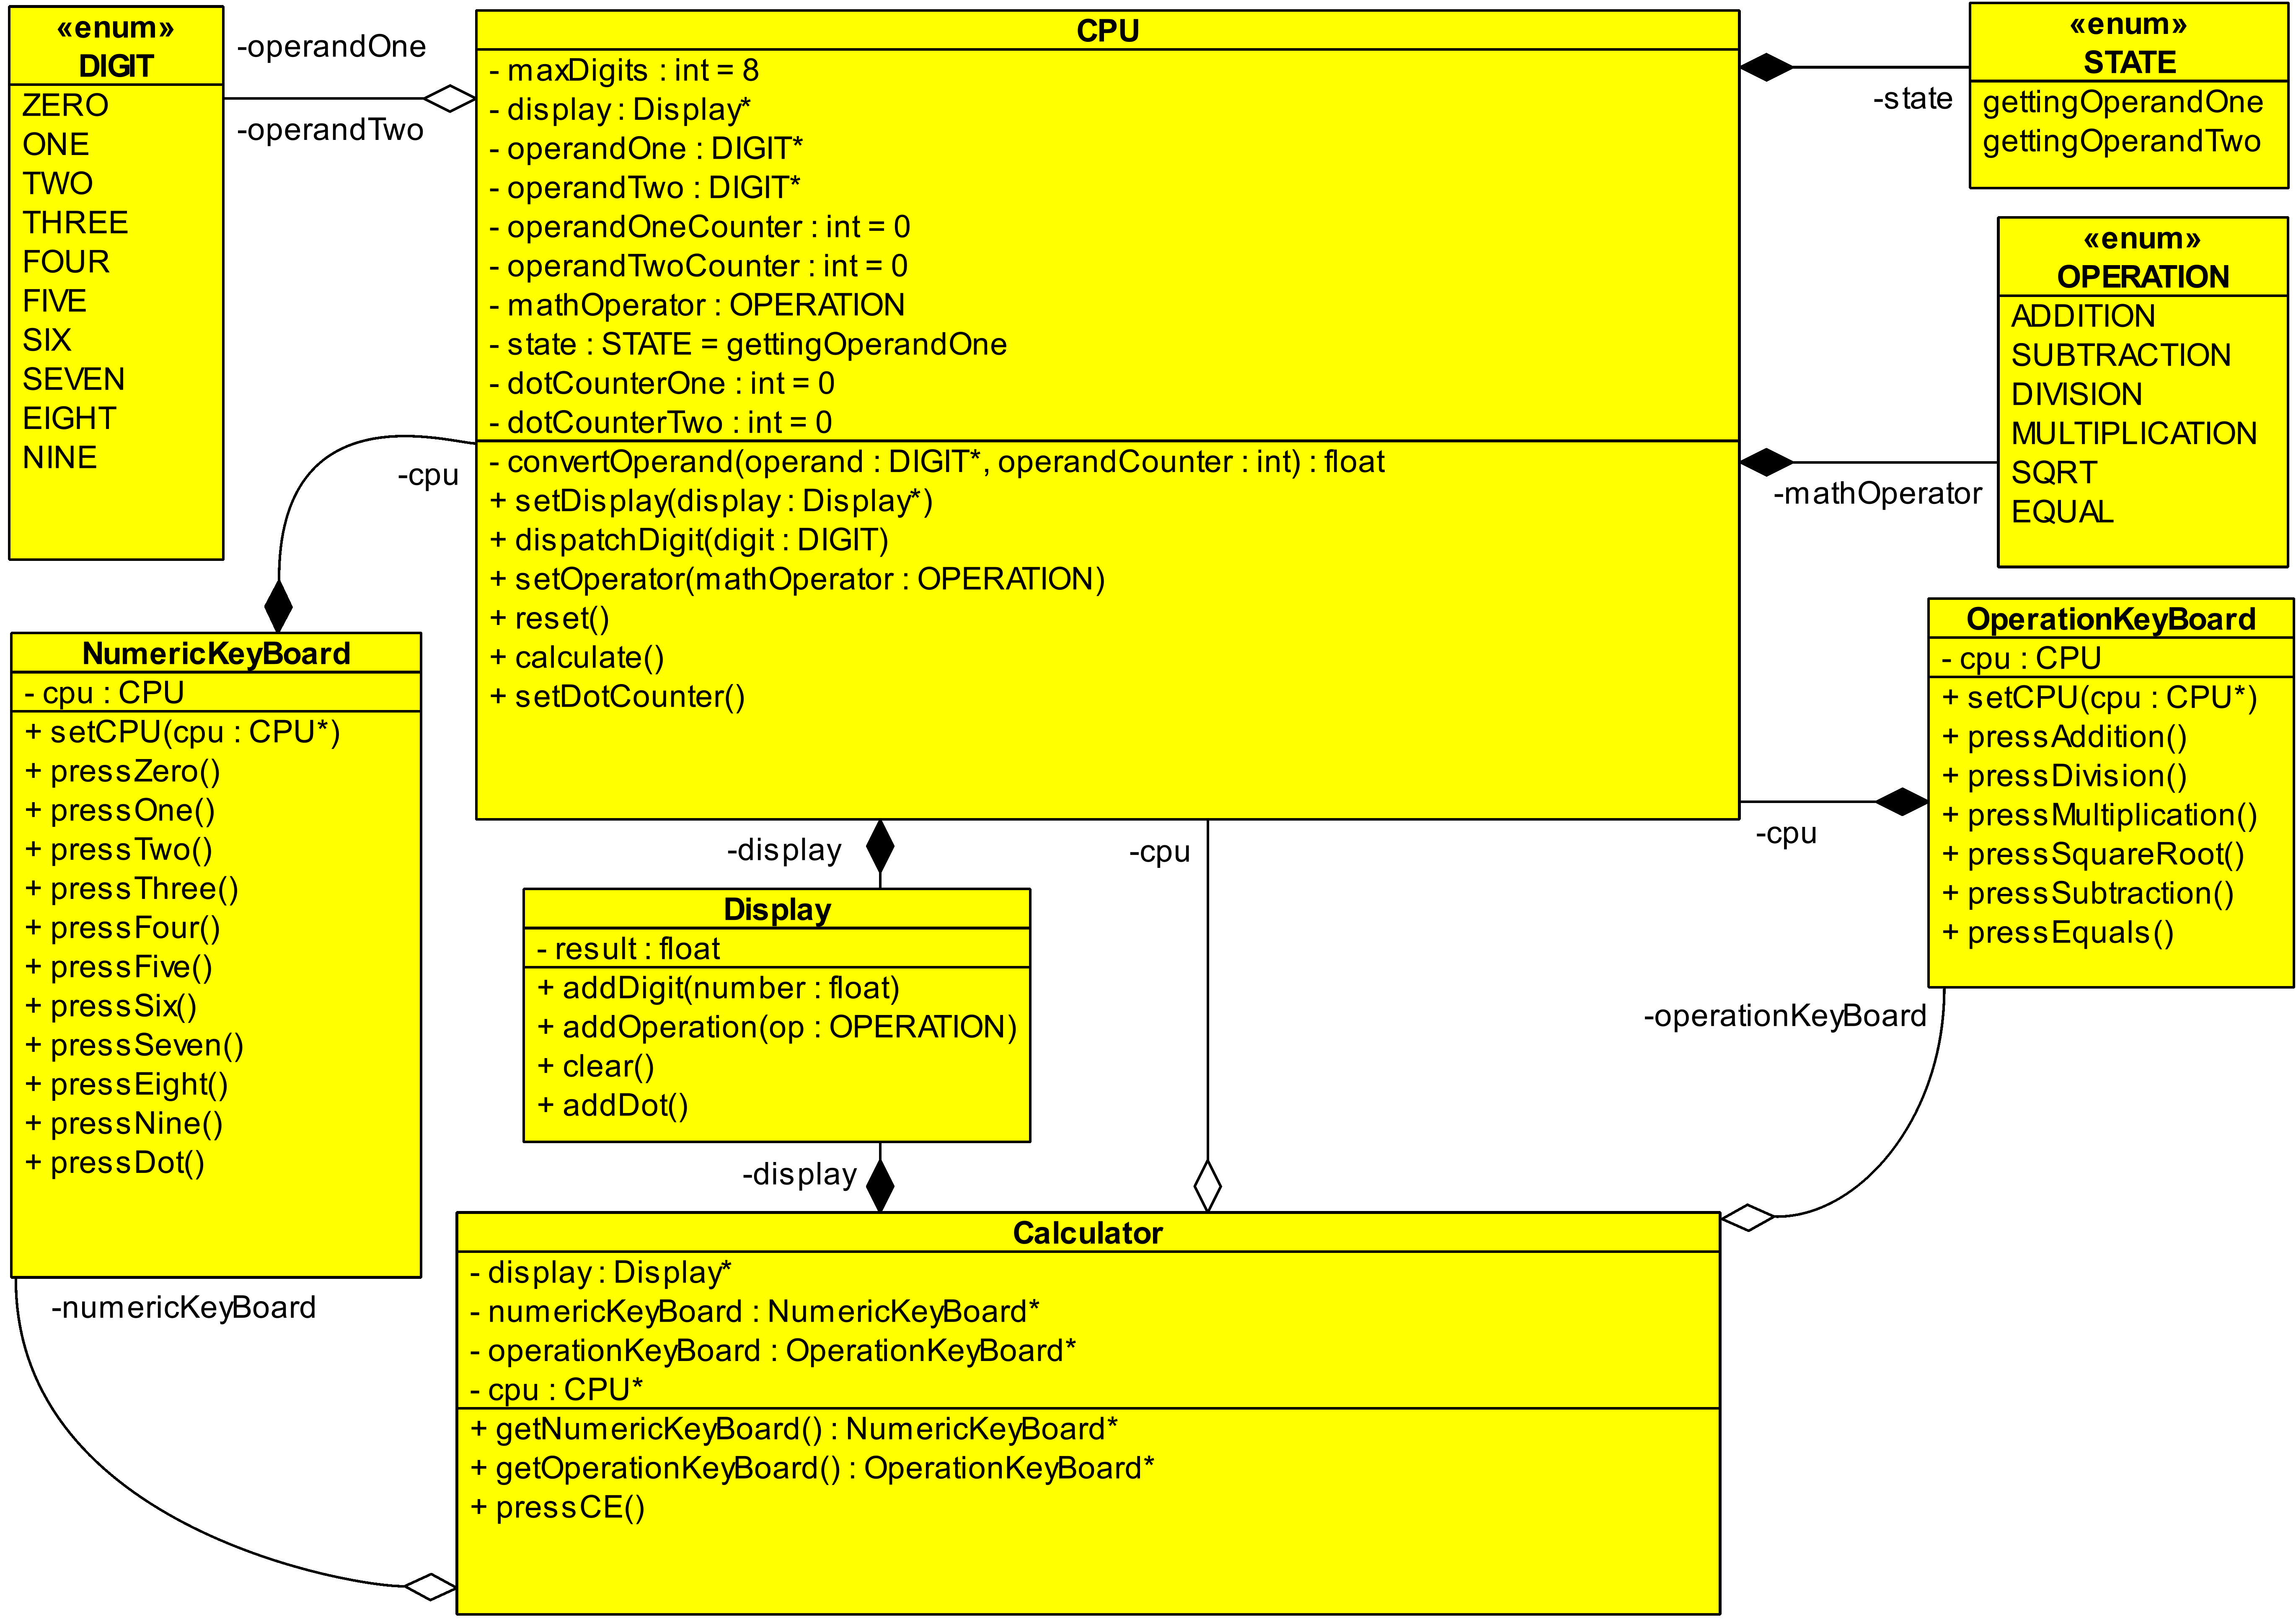
\includegraphics[scale=0.115]{Calculator.png}
		
		\caption{Modelo \textbf{UML} de classe projetado com o software \textit{Umbrello}}
		\label{ModeloClasseUML}
	\end{figure}
\end{document}
